% Pré-requis : afin de tirer bénéfice de ces séances de C/TD/TP, vous devez au préalable maîtriser les savoirs et savoir-faire suivant :
% - connaître les notions de : variable propositionnelle, valuation, modèle, conséquence logique, (in)satisfiabilité
% - utiliser correctement les connecteurs logiques pour la modélisation de problèmes
% - évaluer une conséquence logique, rechercher d'un modèle, tirer les bonnes conclusions quant à  leur (in)existence

% Objectifs : 
% À l'issue de ces séances, vous devrez être capable de transformer un problème de type combinatoire (dont le Sudoku est un exemple typique) en un problème de satisfiabilité d'un ensemble de formules logiques. Pour cela , vous devrez tirer parti des facilités expressives offertes par les connecteurs généralisés dans \touist. Puis, vous devez pouvoir, à partir des modèles obtenus (ou de leur absence) conclure quant aux solutions du problème concret dont vous serez partis.

%Dans cette section, nous nous employons à décrire pas à pas les aspects importants de \touist.

\section{Introduction des fonctionnalités du langage \touist}\label{chap:touist:touist}

%\touist raisonne sur des formules. Ces formules sont un assemblage de \emph{variables propositionnelles} (que nous notons $p$, $q$, $r$\dots) qui représentent des faits du monde réel ainsi que d'opérateurs (que nous appellerons \enquote{connecteurs}) notés $\neg$, $\wedge$, $\vee$, $\Rightarrow$ et $\Leftrightarrow$.

%L'idée est de décrire les contraintes et faits du monde réel à l'aide d'une formule, puis de vérifier les propriétés logiques de cette formule à l'aide du bouton \enquote{Résoudre}. Celui-ci ne permet qu'une chose : vérifier si la formule admet un modèle, c'est à dire que l'affectation de chaque variable propositionnelle (qu'on appellera \enquote{valuation} ou \enquote{interprétation}) permet de rendre l'ensemble de la formule vraie. Si c'est le cas, \touist montrera une telle affectation des variables propositionnelles (que nous appellerons \enquote{modèle}).

Nous présentons maintenant comment utiliser \touist pour vérifier des propriétés essentielles de formules ou d'ensembles de formules logiques, comme la satisfiabilité, la validité ou la conséquence logique.

\paragraph{Vérifier la satisfiabilité d'une formule propositionnelle} Une formule est satisfiable si et seulement si il existe au moins un modèle. Elle est insatisfiable dans le cas où il n'existe aucun modèle et elle est valide si toutes ses valuations possibles sont des modèles.

Par exemple, nous pouvons vérifier que chacun des modèles de la formule suivante ne possède qu'une variable valuée à vrai :

% (p or q or r) and (p => not q) and (q => not r) and (r => not p)
\[(p \vee q \vee r) \wedge (p \rightarrow \neg q) \wedge (q \rightarrow \neg r) \wedge (r\rightarrow \neg p)\]

\noindent
Nous la traduisons d'abord en langage \touist :

\begin{lstlisting}[language=touist,frame=single]
(p or q or r) and (p => not q)
    and (q => not r) and (r => not p)
\end{lstlisting}

\begin{center}
    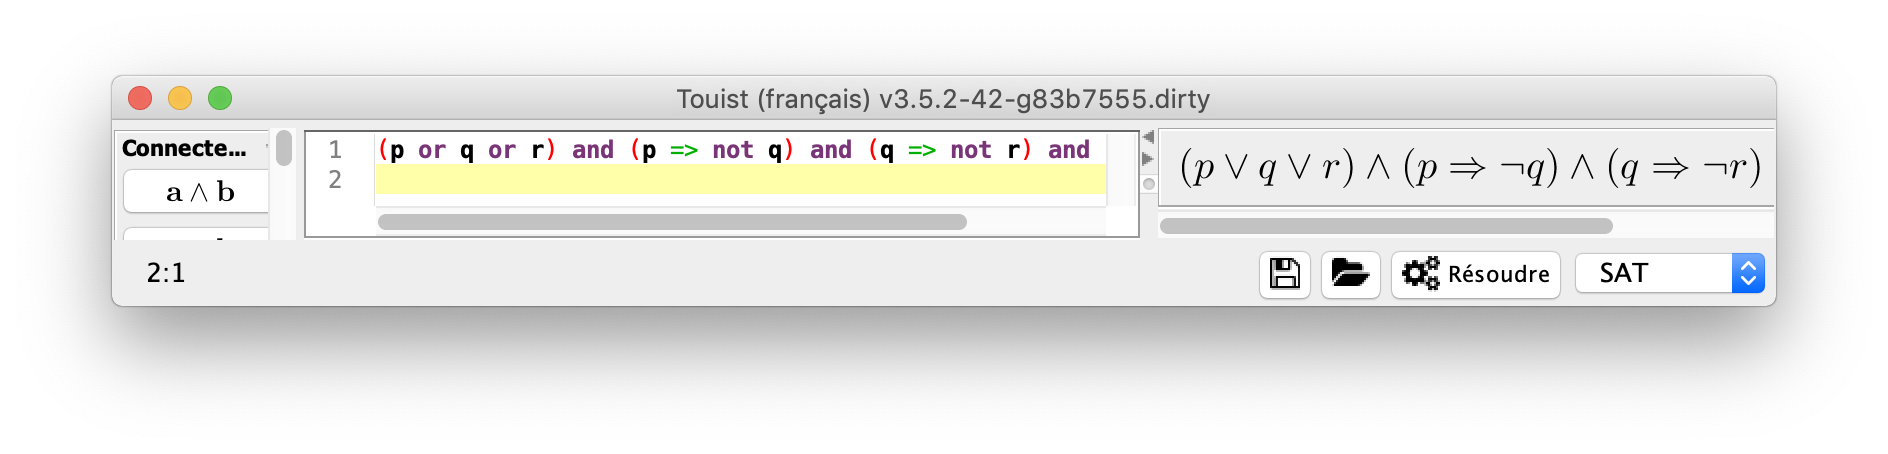
\includegraphics[width=\textwidth]{figures/screenshot-formule.png}
\end{center}

\noindent
Puis, en appuyant sur \enquote{Résoudre}, on obtient le premier modèle :

\begin{center}
    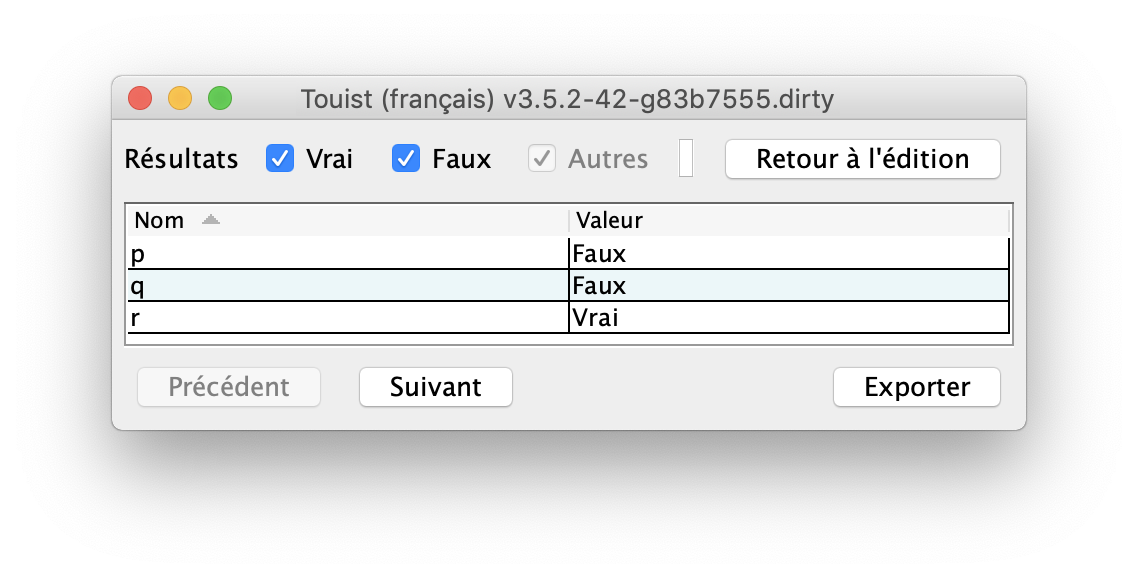
\includegraphics[width=0.5\textwidth]{figures/screenshot-modele.png} \label{fig:screenshot-modele}    
\end{center}

\noindent
En parcourant les modèles suivants avec le bouton \enquote{Suivant}, on constate bien une unique variable propositionnelle vraie par modèle.

\paragraph{Vérifier si un ensemble de formules est satisfiable}

On peut aussi chercher la satisfiabilité d'un ensemble de formules $\phi_i$, noté \[\{\phi_1, \phi_2, \dots\}\]

\noindent
De façon similaire à la satisfiabilité d'une formule, la satisfiabilité d'un ensemble de formules se réduit à déterminer l'existence d'un modèle satisfaisant l'ensemble des formules. Dans \touist, une ensemble de formule est matérialisé par des retour à la ligne : on saisit simplement les formules de l'ensemble les unes au-dessus des autres.\\%, puis Solve. \\
Ainsi, pour vérifiez que l'ensemble $\{\mathit{cafe\vee the, \neg the}\}$ est satisfiable, nous écrivons :

\begin{lstlisting}
cafe or the
not the
\end{lstlisting}


\paragraph{Vérifier la validité d'une formule propositionnelle}

Si nous devions vérifier la validité de la formule précédente, il nous faudrait parcourir les modèles un à un et vérifier que l'ensemble de modèles est égal à l'ensemble des valuations possibles pour cette formule. Pour la formule précédente, il n'y a que trois variables propositionnelles, soit $2^3 = 8$ valuations, la tâche est donc toujours possible. Mais dès que la formule contient davantage de variables, nous procédons  indirectement par réfutation.

\noindent
Ainsi, si la formule est valide, sa négation sera insatisfiable. On teste donc sa négation (i.e., on rajoute $\neg$ devant la formule).

Concrètement, le test de validité permet par exemple de vérifier qu'un raisonnement est formellement valide (mais cela n'exclut pas la possibilité de prémisses ou conclusions fausses). Par exemple :
\[pluie \wedge (pluie \rightarrow routeMouillee) \wedge (routeMouillee \rightarrow danger) \rightarrow danger\]

\noindent En \touist, cela donne :

\begin{lstlisting}[language=touist, frame=single]
pluie and (pluie => routeMouillee)
    and (routeMouillee => danger) => danger
\end{lstlisting}

%\lstinline[columns=fixed,language=touist]{bigand}


%\mael{ --------------- CONTINUER A PARTIR D'ICI ----------}



\paragraph{Vérifier si une formule $C$ est conséquence logique d'un ensemble $H$ de formules}
Supposons que $H=\{H_1,\cdots,H_n\}$ est un ensemble de $n$ hypothèses.\\
Là encore, il serait fastidieux de vérifier que $C$ est vraie dans tous les modèles de $H$. Là encore on procède indirectement en utilisant le théorème : 
\[H\models C \mbox{ si et seulement si } H\cup\{\neg C\}\mbox{ est insatisfiable}\]
autrement dit, pour vérifier si $H\models C$, on va tester si les formules $H_1$, $H_2$,\ldots, $H_n$, $\neg C$ prises \emph{toutes ensemble} sont satisfiables. Si ça n'est pas le cas on pourra conclure que $H\models C$. Si c'est le cas, on aura au moins un contre-modèle ($\sim$ un contre-exemple) qui nous dira dans quelle situation on a les hypothèses vraies et la conclusion fausse.\\


%Exercice : Testez les conséquences suivantes et donnez un contre-modèle quand elle ne sont pas correctes : 
%\begin{itemize}
%\item $f\rightarrow m, f \models m$
%\item $f\rightarrow m, r\rightarrow m, \neg f\wedge \neg r \models \neg m$\\
%(f=j'ai de la fièvre, r=j'ai des rougeurs, m=je suis malade)
%\item $f\rightarrow m, r\rightarrow m, \neg m\models \neg f\wedge \neg r $

%\item 
\noindent Par exemple, supposons que nous avons l'ensemble $H$ de règles et faits suivants :

\begin{enumerate}
\item Si le patient a la rougeole, il a de la fièvre.
\item Si le patient a une hépatite, mais pas la rougeole, il a le teint jaune.
\item Si le patient a de la fièvre ou le teint jaune, il a une hépatite ou la rougeole.
\item Le patient n’a pas le teint jaune.
\item Le patient a de la fièvre.
\end{enumerate}

Nous voulons vérifier que $H\models \mathit{rougeole}$. % dans tous les modèles de $H$, la variables $r$ (correspondant à "le patient a la rougeole") est à "vrai". 
Pour celà, nous pouvons vérifier que l'ensemble de formules suivant, écrit en \touist, est insatisfiable :

\begin{lstlisting}
rougeole => fievre
hepatite and (not rougeole) => teintjaune
fievre or teintjaune => hepatite or rougeole
not teintjaune
fievre
not rougeole
\end{lstlisting}

%\end{itemize}


%\newpage
%\paragraph{Les connecteurs généralisés : $\bigwedge_{i \in A}$ et $\bigvee_{i \in A}$}

\subsection{Résolution de problèmes simples avec SAT}\label{chap:touist:touist:sat-statique}

\paragraph{Les connecteurs généralisés $\displaystyle\bigwedge_{i \in A}$ et $\displaystyle\bigvee_{i \in A}$}~\\

Pour simplifier l'écriture de certaines formules, il est possible d'utiliser des connecteurs logiques généralisés.
Par exemple, considérons une grille de \emph{carré latin}\footnote{comme un sudoku sans la contrainte sur les régions : 1 chiffre par case qui apparaît une seule fois par ligne et par colonne.} $4\times 4$ à résoudre :
\begin{center}
\texttt{
\begin{tabular}{|c|c|c|c|}
	\hline
	~ & ~ & 1 & ~ \\ \hline
	~ &~ & ~ & 2 \\ \hline
	4 & ~ & ~ & ~ \\ \hline
	~ & ~ & 3 &  \\ \hline
\end{tabular}
}\\
\end{center}

Pour chacune des cases, nous définissons quatre variables propositionnelles correspondant aux quatre valeurs possibles $\{1,2,3,4\}$ qu'on écrit aussi $[1..4]$. Ainsi, $p(i,j,k)$ représentera la proposition "La case de coordonnées $(i,j)$ contient la valeur $k$".\\

Pour imposer que la case de coordonnées (2,1) contient l'une des quatre valeurs possibles, nous pouvons utiliser la formule : \\
\[\texttt{p(2,1,\hl{1}) or p(2,1,\hl{2}) or p(2,1,\hl{3}) or p(2,1,\hl{4})}\]

Cette succession de $\vee$ ou seul l'un des indices (surligné) varie peut être condensée en utilisant la disjonction généralisée :%le $\bigvee$ : 
\[\bigvee_{k\in [1..4]} \texttt{p(2,1,\hl{k})} \]
qui signifie donc "la case (2,1) contient l'une des quatre valeurs possibles", ou "pour l'une au moins des quatre valeurs possibles, cette valeur est dans la case (2,1)". \\

\noindent Nous pouvons remarquer l'analogie avec le $\Sigma$ mathématique avec lequel une expression telle que : 
\[f(x,1)+f(x,2)+\cdots+f(x,10)\]
serait condensée en :
\[\sum_{k\in[1..10]} f(x,k)\]


Nous voulons maintenant exprimer que \emph{toutes} les cases de la ligne 2 (cases de coordonnées (2,x)) contiennent l'une des quatre valeurs possibles : 

\[\bigvee_{k\in [1..4]} \texttt{p(2,\hl{1},k)} \wedge \bigvee_{k\in [1..4]} \texttt{p(2,\hl{2},k)}\wedge
\bigvee_{k\in [1..4]} \texttt{p(2,\hl{3},k)} \wedge
\bigvee_{k\in [1..4]} \texttt{p(2,\hl{4},k)}\] 

Pour cela, nous utilisons la conjonction généralisée %le $\bigwedge$ 
en faisant varier l'indice surligné et obtenons : 
\[\bigwedge_{j\in [1..4]}\bigvee_{k\in [1..4]} \texttt{p(2,\hl{j},k)}\]

Ce qui peut se lire "pour chaque case de la ligne 2, pour au moins une valeur de [1..4], cette valeur est dans la case".\\

Afin maintenant d'exprimer la même chose pour chaque ligne, nous généralisons en faisant varier le numéro de ligne : 
\[\begin{matrix}\displaystyle\bigwedge_{j\in [1..4]}\bigvee_{k\in [1..4]} \texttt{p(\hl{1},j,k)}\wedge \bigwedge_{j\in [1..4]}\bigvee_{k\in [1..4]} \texttt{p(\hl{2},j,k)}\\\displaystyle\wedge \bigwedge_{j\in [1..4]}\bigvee_{k\in [1..4]} \texttt{p(\hl{3},j,k)}\wedge \bigwedge_{j\in [1..4]}\bigvee_{k\in [1..4]} \texttt{p(\hl{4},j,k)}\end{matrix}\]

soit, en utilisant à nouveau la conjonction généralisée :%le $\bigwedge$ :

\[\bigwedge_{i\in [1..4]}\bigwedge_{j\in [1..4]}\bigvee_{k\in [1..4]} \texttt{p(\hl{i},j,k)}\]
Qui peut se lire "Pour chaque case (i,j) de la grille, il y a au moins une valeur parmi les quatre possibles qui y figure". \\

\noindent NB : sans ces facilités d'écriture, il aurait fallu 64 propositions et 63 connecteurs pour écrire la même chose. \\

\noindent Cette écriture est possible dans \touist en utilisant des variables \texttt{\$i}, \texttt{\$j} et \texttt{\$k} :

%Ce qui donne : 
\begin{lstlisting}
bigand $i in [1..4]:
  bigand $j in [1..4]:
    bigor $k in [1..4]:
      p($i,$j,$k)
    end
  end
end
\end{lstlisting}

% \begin{center}
% 	\begin{tabular}{cV{4cm}} \toprule
% 		Logique propositionnelle & Langage \touist \\ \midrule
% 		Pour $n\in \mathbb{N}^{*}$, $\underset{i\in [1..n]}{\bigwedge}p_{i}$ & 
% 		\begin{verbatim}
% 		bigand $i in [1..n]:
% 		    p($i)
% 		end
% 		\end{verbatim}
% 		\\ \hline
% 		Pour $n\in \mathbb{N}^{*}$, $\underset{i\in [1..n]}{\bigvee}p_{i}$ & 
% 		\begin{verbatim}
% 		bigor $i in [1..n]:
% 		    p($i)
% 		end
% 		\end{verbatim}
%          \\ \hline
% 	\end{tabular}
% \end{center}

Pour résoudre le carré latin $4\times 4$ donné en exemple, il faut aussi écrire une formule qui impose que chaque cellule contienne au plus une valeur parmi $[1..4]$. Si une cellule contient une valeur alors elle n'en contient pas d'autre. Par exemple, pour exprimer que la case $(1,4)$ contient seulement un 3, il faut parvenir à écrire une formule disant que toute autre valeur que 3 est absente de la case $(1,4)$ : 
\[\texttt{p(1,4,\hl{3}) => (not p(1,4,\hl{1}) and not p(1,4,\hl{2}) and not p(1,4,\hl{4})})\]


On remarque qu'en partie droite de cette implication, on retrouve toutes les valeurs possibles sauf 3. Le langage de \touist permet d'exprimer cela de manière compacte dans une conjonction généralisée grâce à la clause \texttt{when}: 

%\[\texttt{p(1,4,3) => bigand \$k in [1..4] \hl{when \$k!= 3}: not p(1,4,\$k) end}\]
\begin{lstlisting}
p(1,4,3) => bigand $k in [1..4] when $k != 3:
              not p(1,4,$k)
            end
\end{lstlisting}

\noindent De manière générale \texttt{\$i} ne prendra pas la valeur qu'a \texttt{\$j} dans : 
\begin{lstlisting}
   ....
   bigand $i in [1..4] when $i != $j : ....
\end{lstlisting}

Le même principe peut être utilisé pour imposer qu'il n'y ait au plus qu'une fois une même valeur pour chaque ligne et chaque colonne.

Pour passer au sudoku $4\times 4$, il est possible dans \touist d'effectuer des opérations arithmétiques sur des variables entières (par exemple \texttt{p(\$u+\$i,\$v+\$j,\$k)}). Ceci permet d'écrire de manière simple une formule qui interdit deux valeurs identiques dans les cellules d'une même région.
    
%\fred{Sudoku classique ($9\times 9$), résoudre \href{http://puzzling.stackexchange.com/questions/252/how-do-i-solve-the-worlds-hardest-sudoku}{celui-ci par exemple} (l'un des plus difficiles au monde).}

\paragraph{Les ensembles}

Nous avons vu comment définir des variables entières utilisées comme indices.
Nous allons maintenant voir comment utiliser des ensembles génériques pour construire des formules avec les connecteurs généralisés. L'intérêt sera notamment de séparer les règles de résolution d'un problème qui seront définies par des formules permettant de résoudre tout problème de même nature, et des ensembles définissant un problème particulier. Par exemple, dans le cas du Sudoku, les formules permettront de résoudre n'importe quel Sudoku, et les ensembles définiront la grille de Sudoku que nous souhaitons résoudre en particulier.

Par exemple, si nous souhaitons remplacer les chiffres contenus dans les cases du Sudoku par des lettres, nous pouvons alors définir l'ensemble $L=\{A,B,C,D\}$ par \texttt{\$L=[A,B,C,D]} et remplacer \texttt{\$k in [1..4]} par \texttt{\$k in \$L} dans les formules.\\


%Exercice : résoudre le sudoku $4\times 4$ : 

%\begin{center}
%\texttt{
%\begin{tabular}{|c|c|c|c|}
%	\hline
%	A & B & ~ & ~ \\ \hline
%	~ & D & ~ & ~ \\ \hline
%	~ & ~ & A & ~ \\ \hline
%	~ & ~ & C & B \\ \hline
%\end{tabular}
%}\\
%\end{center}

\noindent Voici un codage complet pour cette version du Sudoku. La grille peut être facilement en utilisant les ensembles \texttt{\$x($i$,$j$)} correspondant au contenu initial des cases $(i,j)$:

\begin{lstlisting}
$R = 2
$N = $R * $R
$L = [A,B,C,D]

$x(1,1)=[ ] $x(1,2)=[ ] $x(1,3)=[A] $x(1,4)=[ ]
$x(2,1)=[ ] $x(2,2)=[ ] $x(2,3)=[ ] $x(2,4)=[B]
$x(3,1)=[D] $x(3,2)=[ ] $x(3,3)=[ ] $x(3,4)=[ ]
$x(4,1)=[ ] $x(4,2)=[ ] $x(4,3)=[C] $x(4,4)=[ ]

bigand $i in [1..$N]:
  bigand $j in [1..$N]:
    bigand $k in $x($i,$j):
      p($i,$j,$k)
    end
  end
end

;; au moins une lettre par case
bigand $i in [1..$N]:
  bigand $j in [1..$N]:
    bigor $k in $L:
      p($i,$j,$k)
    end
  end
end
\end{lstlisting}

\begin{lstlisting}
;; au plus une lettre par case
bigand $i in [1..$N]:
  bigand $j in [1..$N]:
    bigand $k1 in $L:
      bigand $k2 in $L$ when $k1!=$k2:
        not p($i,$j,$k1) or not p($i,$j,$k2)
      end
    end
  end
end

;; au plus une fois la meme lettre par ligne
bigand $i in [1..$N]:
  bigand $j1 in [1..$N]:
    bigand $j2 in [1..$N] when $j1!=$j2:
      bigand $k in $L:
        not p($i,$j1,$k) or not p($i,$j2,$k)
      end
    end
  end
end

;; au plus une fois la meme lettre par colonne
bigand $i1 in [1..$N]:
  bigand $i2 in [1..$N] when $i1!=$i2:
    bigand $j in [1..$N]:
      bigand $k in $L:
        not p($i1,$j,$k) or not p($i2,$j,$k)
      end
    end
  end
end

;; au plus une fois la meme lettre par region
bigand $ir in [0..$R-1]:
  bigand $jr in [0..$R-1]:
    bigand $ic1 in [1..$R]:
      bigand $jc1 in [1..$R]:
        bigand $ic2 in [1..$R]:
          bigand $jc2 in [1..$R] when $ic1!=$ic2 or $jc1!=$jc2:
            bigand $k in $L:
              not p($R*$ir+$ic1,$R*$jr+$jc1,$k) or not p($R*$ir+$ic2,$R*$jr+$jc2,$k)
            end
          end
        end
      end
    end
  end
end
\end{lstlisting}


%Exercice : Coloration de cartes.\\

%Le théorème des 4 couleurs, qui fut conjecturé en 1852 par Francis Guthrie, affirme qu'on peut colorer toute carte géographique en utilisant seulement 4 couleurs tout en veillant à ce que deux pays limitrophes reçoivent des couleurs différentes. Il a été (enfin) démontré en 1976 par Appel et Haken. La démonstration a exigé l'usage de l'ordinateur pour étudier les 1478 cas critiques (plus de 1200 heures de calcul à l'époque). \\

%Soit l'ensemble de pays européens (on ne les considère pas tous, mais vous pouvez) : \\
%\begin{multline}
%P = \{Portugal, Espagne, France, Italie, Suisse, Belgique, PaysBas, Pologne, Autriche,\\ RepTcheque, Slovenie, Croatie, Luxembourg, Allemagne\}
%\end{multline}
%Formalisez le problème de la coloration de pays : 
%\begin{itemize}
%\item Chaque pays reçoit une et une seule couleur
%\item Deux pays limitrophes reçoivent des couleurs différentes
%\item Si A est limitrophe avec B, alors B l'est avec A. 
%\end{itemize}
%Vous définirez l'ensemble $P$ des pays et l'ensemble $C$ des couleurs (disons $\{Jaune, Rouge, Vert, Bleu\})$. \\

%\noindent Vous utiliserez les propositions : 
%\begin{itemize}
%\item \texttt{r(p,c)} : "le pays p reçoit la couleur c"
%\item \texttt{l(p1,p2)} : "le pays p1 est limitrophe avec le pays p2"
%\end{itemize}

%NB : en cas de doute, pour savoir lesquels de ces pays sont limitrophes, consultez \href{https://upload.wikimedia.org/wikipedia/commons/6/6a/Europe_countries_map_fr.png}{cette carte}. \\

%Utilisez \touist pour découvrir une solution à quatre couleurs. Puis testez s'il existe une solution à trois couleurs. 


\subsection{Traitement des aspects dynamiques : le jeu de Nim}\label{chap:touist:touist:sat-dynamique}%\label{sec:prob}
Jusqu'ici, nous avons traité de problèmes combinatoires statiques : la solution ne nécessite pas d'ordonner une série d'éléments contrairement à ce qui se passe par exemple dans un jeu où il ne suffit pas de savoir quels coups seront joués mais aussi dans quel ordre. 

Un système qui nécessite la prise en compte de quelque chose (à définir) qui évolue est appelé \emph{système dynamique}. Le système évolue donc en passant d'un \emph{état} à un autre, chaque état pouvant être décrit à l'aide d'une formule logique\footnote{On parle aussi de système de transition ou de système à état discret.}. Une des façons d'en rendre compte est de rendre explicite le déroulement du temps, en général un temps discret qui s'incrémente de 1 entre deux états. Mais on peut aussi en rendre compte tout simplement en nommant les états successifs, le passage du temps étant marqué par le nom des actions effectuées.
Pour illustrer ces aspects dynamiques, nous allons maintenant décrire le déroulement d'une partie de jeu de Nim.


